\documentclass{article}
\usepackage{tikz}
\usetikzlibrary{intersections}
\usetikzlibrary{arrows, decorations.pathmorphing, backgrounds, fit, positioning, arrows.meta, angles, quotes, petri}
\tikzset{help lines/.style=very thin}
\tikzset{Karl's grid/.style={help lines, color=#1!50},
         Karl's grid/.default=blue}
\begin{document}
\section{Karl's graph}

  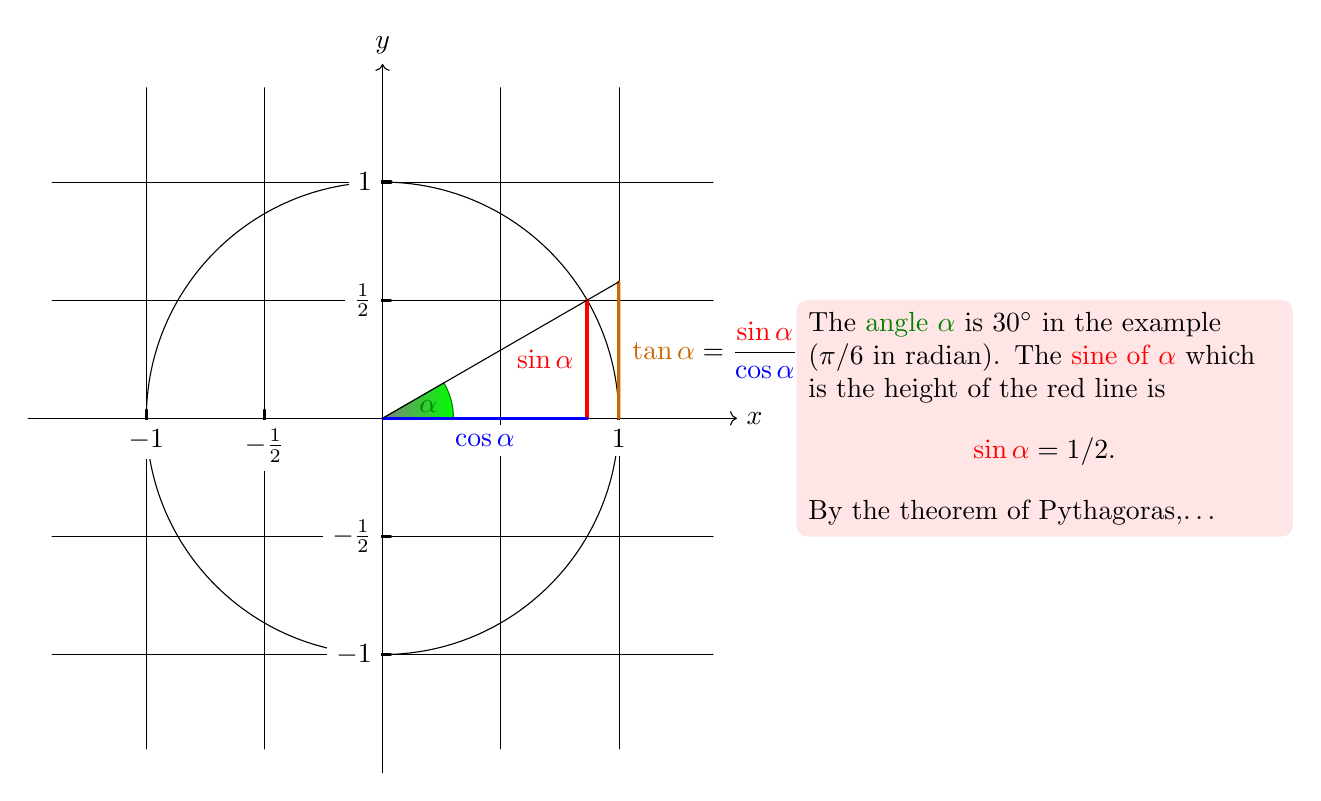
\begin{tikzpicture}[scale=3, line cap=round,
    %Style
    axes/.style=,
    important line/.style={very thick},
    information text/.style={rounded corners,fill=red!10,inner sep=1ex}]
    %Colors
    \colorlet{anglecolor}{green!50!black}
    \colorlet{sincolor}{red}
    \colorlet{tancolor}{orange!80!black}
    \colorlet{coscolor}{blue}
    %\draw[Karl's grid=red] (0,0) grid (5,5);
    %The graphic
    \draw[step=0.5cm, help lines] (-1.4,-1.4) grid (1.4,1.4);

    \draw (0,0) circle [radius=1cm];

    \begin{scope}[axes]
      \draw[->] (-1.5,0)--(1.5,0) node[right]{$x$} coordinate (x axis);
      \draw[->] (0,-1.5)--(0,1.5) node[above]{$y$} coordinate (y axis);
      \foreach \x/\xtext in {-1, -0.5/-\frac{1}{2}, 1}
        \draw[very thick] (\x cm,-1pt)--(\x cm,1pt) node[below=3pt,fill=white]{$\xtext$};
      \foreach \y/\ytext in {-1, -0.5/-\frac{1}{2}, 0.5/\frac{1}{2}, 1}
        \draw[very thick] (-1pt,\y cm)--(1pt,\y cm) node[left=3pt,fill=white]{$\ytext$};
    \end{scope}


    \shadedraw[left color=gray,right color=green,draw=anglecolor] (0,0)--(3mm,0mm)
      arc [start angle=0, end angle=30, radius=3mm]--cycle;
    \draw (15:2mm) node[anglecolor]{$\alpha$};
    % \filldraw[fill=green!20!white, draw=green!50!black] (0,0)--(3mm,0mm)
    %   arc [start angle=0, end angle=30, radius=3mm]--cycle;
    \draw[important line, sincolor] (30:1cm) -- node[left=1pt,fill=white]{$\sin \alpha$}  (30:1cm |- x axis); %+(0,-0.5);

    \draw[important line, coscolor] (30:1cm |- 0,0) -- node[below=2pt,fill=white]{$\cos \alpha$} (0,0); %(30:1cm) ++(0,-0.5) -- (0,0);

    \path [name path=upward line] (1,0) -- (1,1);
    \path [name path=sloped line] (0,0) -- (30:1.5cm);
    \draw [name intersections={of=upward line and sloped line, by=x}]
      [important line, tancolor] (1,0) -- node[right=1pt,fill=white]
      {$\displaystyle \tan \alpha \color{black}=
        \frac{\color{red}\sin \alpha}{\color{blue}\cos \alpha}$} (x);
    %\draw[red, very thick] (30:1cm)--(30:1cm |- 0,0)--(0,0);
    \draw (0,0) -- (x);

    \draw[xshift=1.75cm]
     node[right,text width=6cm,information text]
     {
     The {\color{anglecolor} angle $\alpha$} is $30^\circ$ in the example ($\pi/6$
     in radian). The {\color{sincolor} sine of $\alpha$} which is the height of the red line is
     \[
      {\color{sincolor} \sin \alpha} = 1/2.
     \]
     By the theorem of Pythagoras,\ldots
     };


    % \foreach \x in {-1, -0.5, 1}
    %   \draw[xshift=\x cm] (0pt,-1pt)--(0pt,1pt);
  \end{tikzpicture}
\section{Petri Nets}

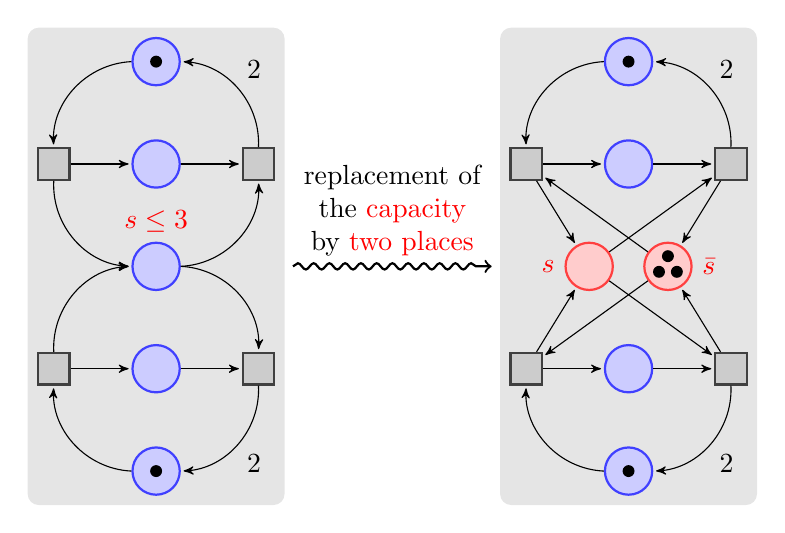
\begin{tikzpicture}
  [
  node distance = 1.3cm, on grid,>=stealth', auto, bend angle = 45,
  % pre/.style={<-,shorten <=1pt,>=stealth',semithick},
  % post/.style={->,shorten >=1pt,>=stealth',semithick},
  every label/.style={red},
  every place/.style={draw=blue!75,fill=blue!20,thick, minimum size = 6mm},
  every transition/.style={draw=black!75,fill=black!20,thick, minimum size = 4mm},
  red place/.style={place,draw=red!75,fill=red!20}
  ]
  \node[place,tokens=1]               (w1)                                          {};
  \node[place]                        (c1)     [below=of w1]                        {};
  \node[place]                        (s)      [below=of c1, label=above:$s\le 3$]  {};
  \node[place]                        (c2)     [below=of s]                         {};
  \node[place,tokens=1]               (w2)     [below=of c2]                        {};

  \node[transition] (t1) [right=of c1] {}
    edge [pre]                                  (c1)
    edge [pre,bend left]                        (s)
    edge [post,bend right] node[swap] {2}       (w1);
  \node[transition] (t2) [left=of c1]  {}
    edge [post]             (c1)
    edge [pre,bend left]    (w1)
    edge [post,bend right]  (s);
  \node[transition] (t3) [right=of c2] {}
    edge [pre, bend right]          (s)
    edge [pre]                      (c2)
    edge [post, bend left] node {2} (w2);
  \node[transition] (t4) [left=of c2]  {}
    edge [post,bend left]            (s)
    edge [post]                      (c2)
    edge [pre, bend right]           (w2);

\begin{scope}[xshift=6cm]
  \node[place,tokens=1]              (w1')                                         {};
  \node[place]                       (c1')    [below=of w1']                       {};
  \node[red place]                   (s1')    [below=of c1',xshift=-5mm]
                                              [label=left:$s$]                     {};
  \node[red place,tokens=3]          (s2')    [below=of c1',xshift=5mm]
                                              [label=right:$\bar{s}$]              {};
  \node[place]                       (c2')    [below=of s2',xshift=-5mm]           {};
  \node[place,tokens=1]              (w2')    [below=of c2']                       {};

  \node[transition]                  (e1')    [left=of c1']                        {}
    edge [pre, bend left]                     (w1')
    edge [pre]                                (s2')
    edge [post]                               (c1')
    edge [post]                               (s1');
  \node[transition]                  (l1')    [right=of c1']                       {}
    edge [pre]                                (c1')
    edge [pre]                                (s1')
    edge [post, bend right] node[swap] {2}    (w1')
    edge [post]                               (s2');
  \node[transition]                  (e2')    [left=of c2']                        {}
    edge [pre]                                (s2')
    edge [pre, bend right]                    (w2')
    edge [post]                               (s1')
    edge [post]                               (c2');
  \node[transition]                  (l2')    [right=of c2']                       {}
    edge [pre]                                (c2')
    edge [pre]                                (s1')
    edge [post]                               (s2')
    edge [post, bend left]  node       {2}    (w2');
\end{scope}

\begin{scope}[on background layer]
  \node (r1) [fill=black!10, rounded corners, fit=(w1)(c1)(s)(c2)(w2)(t1)(t2)(t3)(t4)]                {};
  \node (r2) [fill=black!10, rounded corners, fit=(w1')(c1')(s1')(s2')(c2')(w2')(e1')(e2')(l1')(l2')] {};
\end{scope}

\draw[shorten >=1mm, -to, thick, decorate, decoration={snake, post length=2mm, pre=moveto, pre length=1mm, amplitude=.4mm, segment length=2mm}]
 (r1)--(r2) node [above, midway, text width=3cm, align=center]
 {replacement of the \textcolor{red}{capacity} by \textcolor{red}{two places}};


  %\node[red,above] at (semaphore.north) {$s\le 3$};
\end{tikzpicture}

% scrap drawing
Curved Path Construction. \\
  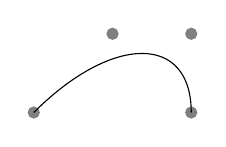
\begin{tikzpicture}
    \filldraw[gray] (0,0) circle [radius=2pt]
                    (1,1) circle [radius=2pt]
                    (2,1) circle [radius=2pt]
                    (2,0) circle [radius=2pt];
    \draw (0,0) .. controls (1,1) and (2,1) .. (2,0);
  \end{tikzpicture}
  \tikz \draw (0,0) circle [radius=10pt];
  \tikz \draw[rotate=30] (0,0) ellipse [x radius=20pt,y radius=10pt];
  \tikz \draw[x=1.57ex,y=1ex] (0,0) sin (1,1) cos (2,0) sin (3,-1) cos (4,0)
                              (0,1) cos (1,0) sin (2,-1) cos (3,0) sin (4,1);
  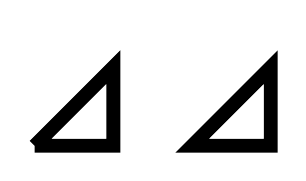
\begin{tikzpicture}[line width=5pt]
    \draw (0,0) -- (1,0) -- (1,1) -- (0,0);
    \draw (2,0) -- (3,0) -- (3,1) -- cycle;
    \useasboundingbox (0,1.5); %make bounding box higher.
  \end{tikzpicture}
  \tikz \shade (0,0) rectangle (2,1) (3,0.5) circle (.5cm); \\
  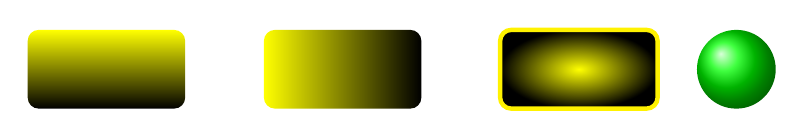
\begin{tikzpicture}[rounded corners, ultra thick]
    \shade[top color=yellow, bottom color=black] (0,0) rectangle +(2,1);
    \shade[left color=yellow, right color=black] (3,0) rectangle +(2,1);
    \shadedraw[inner color=yellow, outer color=black, draw=yellow] (6,0) rectangle +(2,1);
    \shade [ball color=green] (9,0.5) circle (.5cm);
  \end{tikzpicture}
  % difference between + and ++
  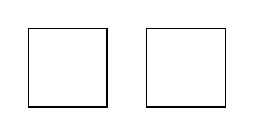
\begin{tikzpicture}
    \def \rectanglepath{-- ++(1cm,0cm)-- ++(0cm,1cm)-- ++(-1cm,0cm)-- cycle}
    \draw (0,0) \rectanglepath;
    \draw (1.5,0) \rectanglepath;
  \end{tikzpicture}
  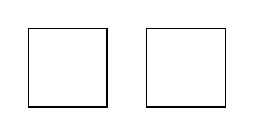
\begin{tikzpicture}
    \def \rectanglepath{-- +(1cm,0cm) -- +(1cm,1cm) -- +(0cm,1cm) -- cycle}
    \draw (0,0) \rectanglepath;
    \draw (1.5,0) \rectanglepath;
  \end{tikzpicture}
  \tikz \draw (0,0) rectangle +(1,1) (1.5,0) rectangle +(1,1);
  % arrow
  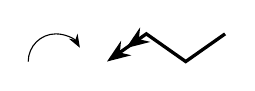
\begin{tikzpicture}[>=Stealth]
    \draw[->] (0,0) arc [start angle=180, end angle=30, radius=10pt];
    \draw[<<-,very thick] (1,0) -- (1.5cm,10pt) -- (2cm,0pt) -- (2.5cm,10pt);
  \end{tikzpicture}
  $?$ Scoping has another interesting effect: Any changes to the clipping area are local to
  the scope. Thus, if you say \verb+\clip+ somewhere inside a scope, the effect of the \verb+\clip+
  command ends after the end of that scope.
  \tikz \draw (0,0) -- (0,0.5) [xshift=2pt] (0,0) -- (0,0.5);
  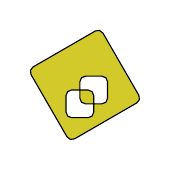
\begin{tikzpicture}[even odd rule, rounded corners=2pt, x=10pt, y=10pt]
    \filldraw[fill=yellow!80!black] (0,0) rectangle (1,1)
          [xshift=5pt, yshift=5pt]  (0,0) rectangle (1,1)
          [rotate=30]             (-1,-1) rectangle (2,2);
  \end{tikzpicture}
  \foreach \x in {1,2,3} {$x=\x$, }
%Venn diagram, Till Tantau
\def\firstcircle{(0,0) circle (1.5cm)}
\def\secondcircle{(45:2cm) circle (1.5cm)}
\def\thirdcircle{(0:2cm) circle (1.5cm)}

% Now we can draw the sets:
\begin{tikzpicture}

    \begin{scope}[even odd rule]
      \clip \secondcircle;
      \clip \firstcircle;
      \clip \thirdcircle (-3,-3) rectangle (3,3);
      \fill[red] \secondcircle;
    \end{scope}
    \draw \firstcircle node[below] {$A$};
    \draw \secondcircle node [above] {$B$};
    \draw \thirdcircle node[below] {$C$};
\end{tikzpicture}
%End of the Venn diagram.
% Drawing a series of circles using TikZ
\\
\tikz \foreach \x in {1,...,10}
        \draw (\x,0) circle [radius=0.4cm];
We can also nest loops to create interesting effects.\\
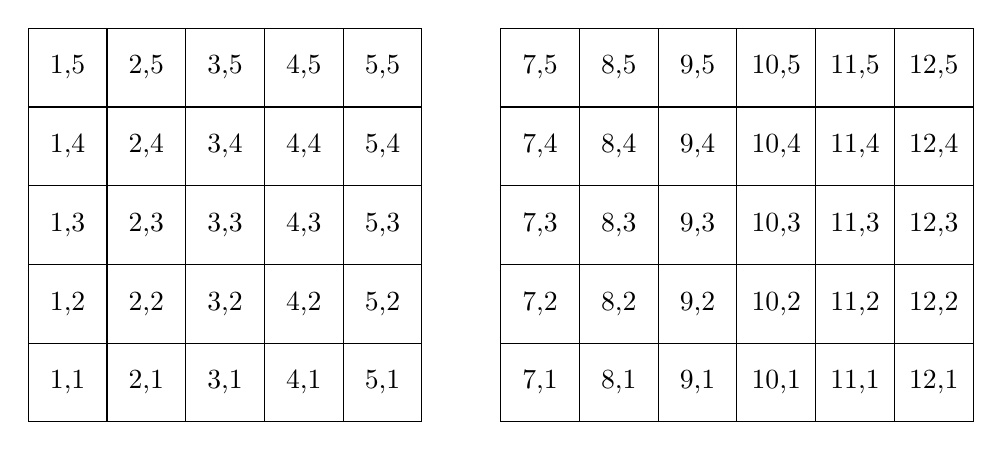
\begin{tikzpicture}
  \foreach \x in {1,...,5,7,8,...,12}
    \foreach \y in {1,...,5}
  {
  \draw (\x,\y) +(-.5,-.5) rectangle +(.5,.5);
  \draw (\x,\y) node{\x,\y};
  }
\end{tikzpicture}

Labeling examples using TikZ.

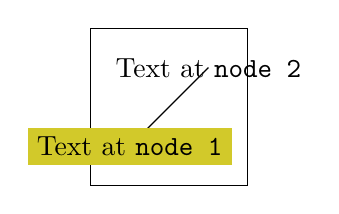
\begin{tikzpicture}
  \draw (0,0) rectangle (2,2);
  \draw (.5,.5) node [fill=yellow!80!black]
                     {Text at \verb!node 1!}
   -- (1.5,1.5) node {Text at \verb!node 2!};
\end{tikzpicture}
You can also position labels on curves and, by adding the \verb!sloped! option,
have them rotated such that they match the line's slope.

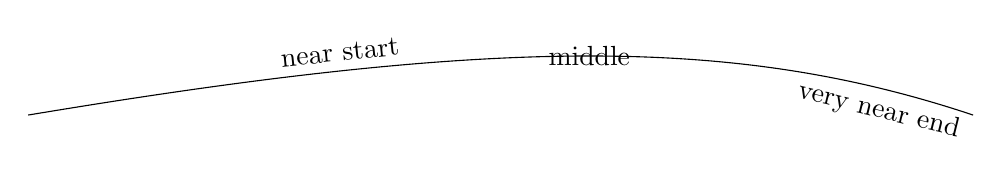
\begin{tikzpicture}
  \draw (0,0) ..controls (6,1) and (9,1)..
       node[near start,sloped,above]{near start}
       node{middle}
       node[very near end,sloped,below]{very near end} (12,0);
\end{tikzpicture}

Using pics to reuse a piece of code in a picture.

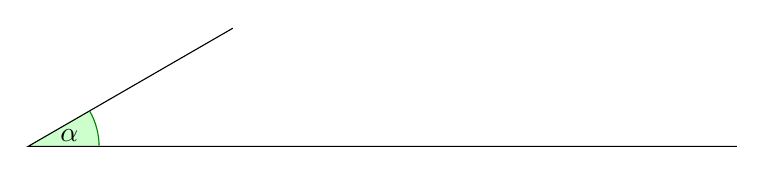
\begin{tikzpicture}[scale=3]
  \coordinate (A) at (3,0);
  \coordinate (B) at (0,0);
  \coordinate (C) at (30:1cm);

  \draw (A) -- (B) -- (C)
  pic[draw=green!50!black,fill=green!20,angle radius=9mm,
  "$\alpha$"]{angle=A--B--C};
\end{tikzpicture}
\end{document}
